\documentclass{mcmthesis}

  \makeatletter
  \newcommand{\rmnum}[1]{\romannumeral #1}
  \newcommand{\Rmnum}[1]{\expandafter\@slowromancap\romannumeral #1@}
  \makeatother

\mcmsetup{CTeX = false,   % 使用 CTeX 套装时,设置为 true
        tcn = 0025, problem = A,
        sheet = true, titleinsheet = true, keywordsinsheet = true,
        titlepage = false, abstract = true}
\usepackage{palatino}
\usepackage{lipsum}
\usepackage{amsmath}  
\usepackage{amssymb}
\usepackage{indentfirst} 

\setlength{\parindent}{1.5em}

\title{The Model of Image Compression and Inpainting}
\begin{document}
\begin{abstract}

The information age brings about "information explosion", which increases the amount of data. Therefore, it is necessary to compress the data effectively, whether it is transmitted or stored.
And digital images need a lot of data. Large amount of data of image information will not only challenge of reservoir storage capacity, puts forward higher requirements on the bandwidth of the communication channel, but also to the processing speed of the computer has brought great pressure, so a good model for image compression is indispensable.
In addition, in the process of information compression, there must be some missing information, and selecting the appropriate method to deal with the loss information is of great significance to the image after the final decompression.

Based on image information loss of compression and recovery, we build a simple image compression model to compress image. And we analysis the loss of image information, with Using the resulting conclusions, selecting an appropriate method to restore the image.

For problem 1, 2, we use a combination of traditional digital image processing methods to make image compression. 
We first convert the RGB color space or grayscale color space into a more lossy YCbCr color space, then use the traditional sampling method.
After that, the image was processed by $8\times 8$ block, combining DCT, quantization table, Zig-Zag, modified RLE and Huffman encoding, etc., to compress image. Such a combination, is more stable and flexible in use, and have a good image compression performance.

For problem 3, we analyze the provided example graph and find that the information shown is similar to the salt and pepper noise. In spatial and frequency domain for different treatment, we find that after adopting the spatial median filter processing the result is best, a then on the basis of the simple model, we have adopted much more flexible adaptive median filter, in response to different degree of missing information.

In this work, we're going to look through the literature, the calculation, the programming, and the other ways to get to know the current mainstream method.
Several models are bulit on the basis of which can meet the requirements of the problem and are simple and easy to implement. They have good processing for the provided example graph processing.
\begin{keywords}
DCT; Huffman Coding; Median Filtering
\end{keywords}
\end{abstract}
\maketitle
\tableofcontents
\newpage
\section{Introduction}
\subsection{Background}

With the rapid development of artificial intelligence, there are more and more applications of images, such as face recognition and automatic recognition. There are two things that cannot be ignored before using images for related tasks.The first is image compression, in order to reduce the redundant information in image data and to store and transmit data in a more efficient format; the second is image restoration, which USES certain techniques to reproduce the missing information in the image.  These two technologies have laid a foundation for the rapid development of relevant image application technologies. In this context, we want to be able to build a process model to implement these two technologies.

\subsection{Restatement of Problem}

We are required to build some mathematical model to process the data of images:
\begin{itemize}
\item A lossy image compression model
\item An inpainting model to recover the image with 20\% missing information.
\item A model to compress a surveillance video in a shopping mall.
\end{itemize}

\subsection{Overview of Our Work}

First, we find a few key points in these questions :
\begin{itemize}
  \item The image compression we need to do is lossy compression.
  \item How to make image compression model suitable for general situation?
  \item What is the relationship between the models we want to build?
  \item Does the missing data proportion have special meaning?
  \item What is the measure of restoration?
  \item All missing pixel values for a given image are non-zero.
  \item How to deal with the static background of video?
\end{itemize}

\section{Assumptions}
\begin{itemize}
  \item We are dealing with bitmaps rather than vectors.
  \item Assume that the missing types of information in question 3 are the same as those in the case diagram.
  \item Assume that the image the image compression algorithm to process is not too extreme for the its size, that is, the image size is not too small or too large.
  \item Assume the image compression algorithm is aimed at the image of RGB color.
  \item Assume that the image compression requires not to lose too much information, not considering the high compression of the signal loss.
\end{itemize}

\section{Notations}

\subsection{Notations}
\begin{table}[htb]
\centering

\begin{tabular}{ll} 
\toprule

Symbol & Specification \\
\toprule
$N$  &  The number of pixels in a horizontal, vertical direction. \\

$Z_{min}$ & The minimum gray value in the window. \\

$Z_{max}$ & The maximum gray value in the window. \\

$Z_{med}$ & The medimum gray value in the window. \\

$Z_{xy}$  & Represents the grayscale value of coordinates (x,y). \\

$S_{max}$ & Maximum window size allowed. \\

$S_{xy}$  & Current window size. \\

$MAX_I$ & The maximum value of the color of the image point. \\


\bottomrule
\end{tabular}
\end{table}

\section{Our Model}
\subsection{Model \Rmnum{1}}
For a digital image using RGB color mode, we first separate the three color channels of red, green and blue.The image data of each channel can be represented by a 2-dimensional matrix. Each element in the 2-dimensional matrix corresponds to one pixel, and its value is the pixel's gray value. After obtaining the three 2-dimensional matrices, We first convert it from RGB to YCbCr. Where Y is the brightness component, Cb is the blue color component, and Cr is the red color component.The human eye is more sensitive to the Y component, so it will be less noticeable to the naked eye when subsampling the chromaticity component to reduce the chromaticity component.YCbCr color space and RGB color space conversion formulas are as follows:
\begin{equation}
\begin{cases}Y=0.299R+0.587G+0.114B\\Cb=0.564(B-Y)\\Cr=0.713(R-Y)\end{cases}
\end{equation}
\begin{equation}
\begin{cases}R=Y+1.402Cr\\G=Y-0.344Cb-0.714Cr\\B=Y+1.772Cb\end{cases}
\end{equation}


We decide use YCbCr 4:2:0 format,which is by far the most common color representation used in compressedimages and video.[1] 
We sampled it in a 4:2:0 format. 4: 0 will correspond to four brightness values with 1 color value. For the first chromaticity element, there are two sample values, and the second chromaticity element will not be sampled. This does not produce a complete color image. In fact, 4:2:0 means that each scan has two color samples, which are sampled every two lines.
This sampling is to reach a certain lossy compression without affecting the visual experience.

We divide them into sub-blocks separately to improve the efficiency of subsequent operations. Our specific operation is to divide the original matrix into sub-blocks of $8\times8$ in order from left to right and from top to bottom. After this step, A sub-block is considered as the basic unit to operate.
There are 2 things to note about blocking:
\begin{itemize}
\item Each value in the 2-dimensional matrix needs to be subtracted by 128 before blocking so that the range of each value in the 2-dimensional matrix is changed from 0 to 255 to -128 to 127.
\item The length or width of the original image is not a multiple of 8, which needs to make up to be multiples of 8 so that the 2-dimensional matrix is completely divided into several sub-blocks.
\end{itemize}
There are 3 advantages to blocking:
\begin{itemize}
  \item To facilitate the DCT.
  \item There are no restrictions on the length-width ratio of the image.
  \item Take into account the local similarity of the picture.  
\end{itemize}

The discrete cosine transform (DCT) is a technique for converting a signal into elementary frequency components. It is widely used in image compression.[2] And our model uses 2-dimensional DCT.The most common DCT definition of a 1-D sequence of length N is 
\begin{equation}
  C(u)=\alpha(u)\sum_{x=0}^{N-1}f(x)\cos\left[\frac{(2x+1)u\pi}{2N}\right]
\end{equation}
for $u$ $=$ 0,1,2...,$N-1$. The inverse transformation is defined as
\begin{equation}
  f(x)=\sum_{x=0}^{N-1}\alpha(u)C(u)\cos\left[\frac{(2x+1)u\pi}{2N}\right]
\end{equation}
for $u$ $=$ 0,1,2...,$N-1$. In both equations (3) and (4) $\alpha(u)$ is defined as 
\begin{equation}
  \alpha(u)=\begin{cases}\sqrt{\frac1N},&\text{for }u=0\\
    \sqrt{\frac2N},&\text{for } u\not= 0
    \end{cases}
\end{equation}
The 2-D DCT is a direct extension of the 1-D case and is given by
\begin{equation}
  C(u,v) = \alpha(u)\alpha(v)\sum_{x=0}^{N-1}\sum_{y=0}^{N-1}f(x,y)\cos\left[\frac{(2x+1)u\pi}{2N}\right]\cos\left[\frac{(2y+1)v\pi}{2N}\right]
\end{equation}
for $u$ $=$ 0,1,2...,$N-1$ and $\alpha(u)$ and $\alpha(v)$ are defined in (5). The inverse transform is defined as 
\begin{equation}
  f(x,y) = \sum_{x=0}^{N-1}\sum_{y=0}^{N-1}\alpha(u)\alpha(v)C(u,v)\cos\left[\frac{(2x+1)u\pi}{2N}\right]\cos\left[\frac{(2y+1)v\pi}{2N}\right]
\end{equation}
for $u$ $=$ 0,1,2...,$N-1$. The 2-D basis functions can be generated by multiplying the horizontally oriented 1-D basis functions with vertically oriented set of the same functions.[3] DCT is the transform of signal from time domain to frequency domain, and its transformation result is not complex, all is real.Each $8\times8$ original pixels is changed into $8\times8$ digits, and each number is composed of original 64 data through the basis function.

The next step is quantization. Quantization here refers to the quantization of the frequency coefficient after FDCT. The aim is to reduce the magnitude of the non-zero coefficient and increase the number of zero coefficients.

\begin{figure}[h]
\centering
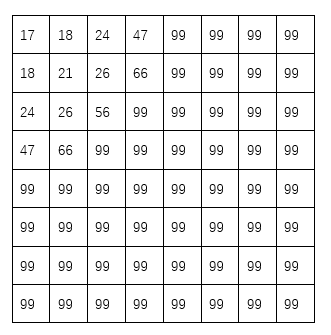
\includegraphics[width=10cm]{lqt.png}
\caption{Luma quantization table} \label{fig: Luma quantization table}
\end{figure} 

\begin{figure}[h]
\centering
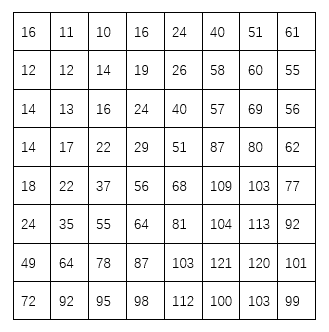
\includegraphics[width=10cm]{cqt.png}
\caption{Chroma quantization table} \label{fig: Chroma quantization table}
\end{figure} 

The quantization that we do is to divide the pixel value by the quantized table.Because the value in the upper left corner of the quantization table is smaller, the value in the upper right corner is larger, the purpose of maintaining low frequency components and suppressing high frequency components is achieved.

After that, Zig-Zag scan is performed on the quantized change coefficient. The so-called Zig-Zag scan is to start from the upper left corner of the matrix and scan according to the shape of the letter 'Z'. The purpose of the scanning is as follows:
\begin{itemize}
  \item To group low frequency coefficients in top of vector. 
  \item  Maps $m\times n$ to a $1\times m*n$ vector.
\end{itemize}

\begin{figure}[h]
\centering
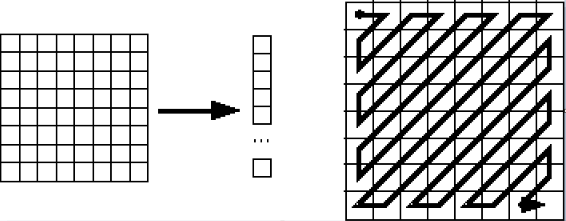
\includegraphics[width=12cm]{Zig-Zag.png}
\caption{Zig-Zag scan} \label{fig:Zig-Zag scan}
\end{figure}

After Zig-Zag scanning, the low-frequency components in this one-dimensional vector are in the front, and the high frequency components are later. It is worth noting that the high frequency component has a large number of continuous zero values, which is making for 0-RLE.

0-RLE is an encoded mode we create which referred to RLE and aimming at zero. RLE(Run-length encoding) is a very simple form of lossless data compression in which runs of data (that is, sequences in which the same data value occurs in many consecutive data elements) are stored as a single data value and count, rather than as the original run. This is most useful on data that contains many such runs. For example, With a RLE data compression algorithm applied to the a character string 'AAAABBB', it can be rendered as follows:'4A3B'. 0-RLE only do special coding for 0, other values are reserved. The specific step is as follows:

Initialize a queue, and the encoder will scan the elements of the vector to the tail. If zero is encountered, the num of zeroes is counted until a non-zero is encountered. If the non-zero value is encountered, zero and its count are pressed into the queue. If the next number is non-zero, the current number is pressed into the queue. When the tail is read, if the value is zero, zero and its count are pressed into the queue; if the value is non-zero, it is pressed into the queue.For example, With a RLE data compression algorithm applied to the a digital string '0 0 1 2 3 0 1 0 0 0 0 0 0 0 1', it can be rendered as follows :'0 2 1 2 3 0 1 1 0 7 1'.

Final, the 1-dimensional vector obtained from last step is encoded with huffman coding.Huffman coding is the basic method of image data scan again and calculate the probability of all pixels appear, according to the size of the probability of different length of code word only, the greater the probability of the pixels shorter code. The result of huffman coding we do is a hoffman collation of the image. The encoded data is the code word corresponding to each pixel, and the corresponding relation between the code word and the actual pixel value is recorded in the code table.

For a set of symbols with a uniform probability distribution and a number of members which is a power of two, Huffman coding is equivalent to simple binary block encoding.

\emph{Input}

Alphabet  ${\displaystyle A=\left\{a_{1},a_{2},\cdots ,a_{n}\right\}}$, which is the symbol alphabet of size ${\displaystyle n}$.

Tuple ${\displaystyle W=(w_{1},w_{2},\cdots ,w_{n})}$, which is the tuple of the (positive) symbol weights (usually proportional to probabilities), i.e. ${\displaystyle w_{i}=\mathrm {weight} \left(a_{i}\right),1\leq i\leq n}$.

\emph{Output}

Code ${\displaystyle C\left(W\right)=(c_{1},c_{2},\cdots ,c_{n})}$, which is the tuple of (binary) codewords, where$ {\displaystyle c_{i}}$ is the codeword for ${\displaystyle a_{i},1\leq i\leq n}$.

\emph{Goal}

Let ${\displaystyle L\left(C\left(W\right)\right)=\sum _{i=1}^{n}{w_{i}\times \mathrm {length} \left(c_{i}\right)}} {\displaystyle L\left(C\left(W\right)\right)=\sum _{i=1}^{n}{w_{i}\times \mathrm {length} \left(c_{i}\right)}} $be the weighted path length of code ${\displaystyle C}$ C. Condition: {\displaystyle L\left(C\left(W\right)\right)\leq L\left(T\left(W\right)\right)} ${\displaystyle L\left(C\left(W\right)\right)\leq L\left(T\left(W\right)\right)} $for any code ${\displaystyle T\left(W\right)}$. 

\begin{figure}[h]
\centering
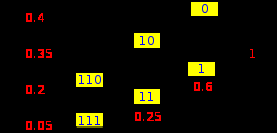
\includegraphics[width=12cm]{Huffman.png}
\caption{Huffman Coding} \label{fig:Huffman Coding}
\end{figure}

For the above steps, the steps before the Zig-Zag scan is a lossy image compression to eliminate data redundancy, which is unble to recover after inverse transform. the steps after the Zig-Zag scan is a lossless image compression to eliminate encoding redundancy, which is able to reduce storage space needed.


\subsection{Model \Rmnum{2}}
\subsubsection{Model proposed}
For problem 3, due to missing data itself is irreversible, we find after the analyses of current situation of the lack of case diagram, as shown in the image information loss and image noise are similar, so this article will be treated as missing data processing as a noise.

Spatial filtering is an enhanced method based on neighborhood processing. Spatial filtering processes directly in the two-dimensional space of the image. In other words, the grayscale value of each pixel is processed. 
It use a template to perform some mathematical operation on all pixels of each pixel and its surround neighborhood to get that new gray value of the pixel. The new grayscale value is not only related to the gray value of the pixel, but also to the gray value of the pixel in the neighborhood.
In this paper, a variety of filters are used and compared. As shown in the figure below, with the same 3X3 template, the median filter is finally found to be suitable for the case diagram.

\begin{figure}[h]
\centering
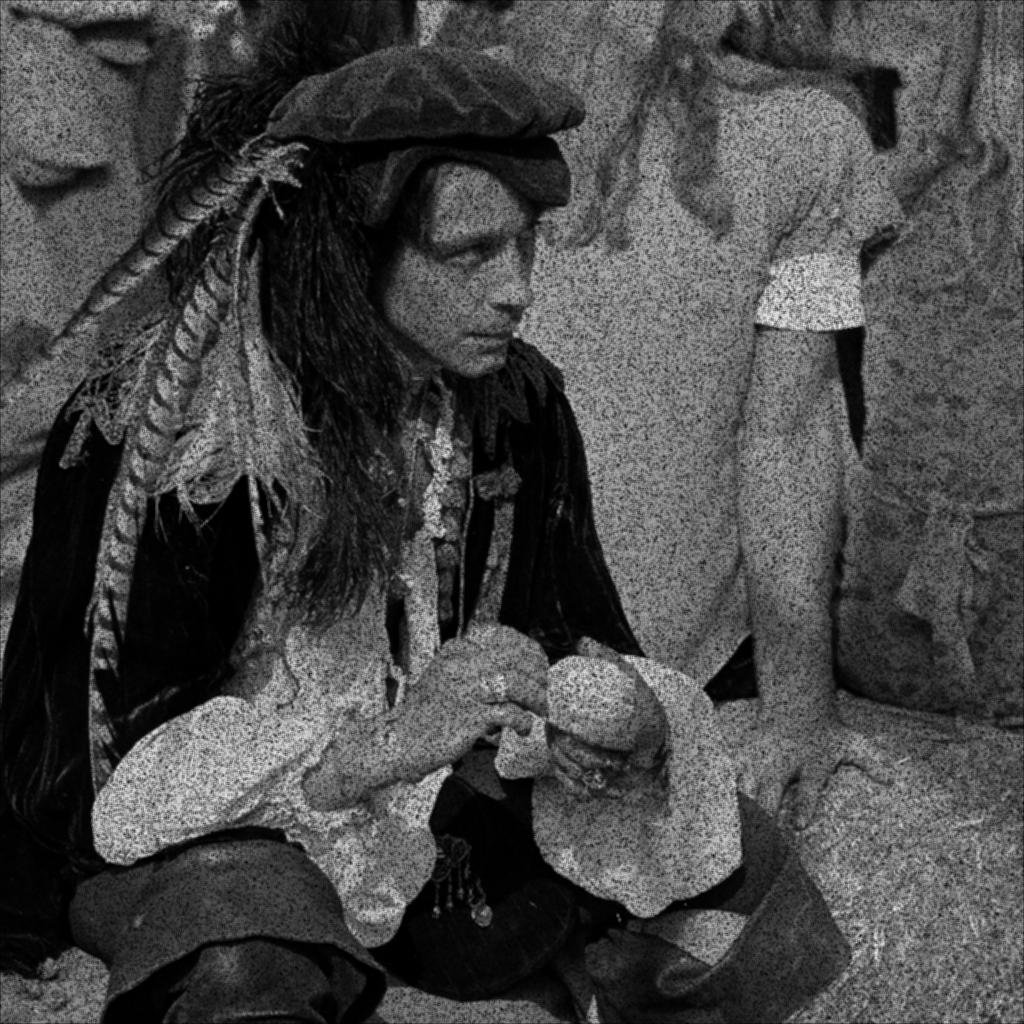
\includegraphics[width=10cm]{WienerFilterting.jpg}
\caption{WienerFilterting} \label{fig: WienerFilterting}
\end{figure}
    

\begin{figure}[h]
\centering
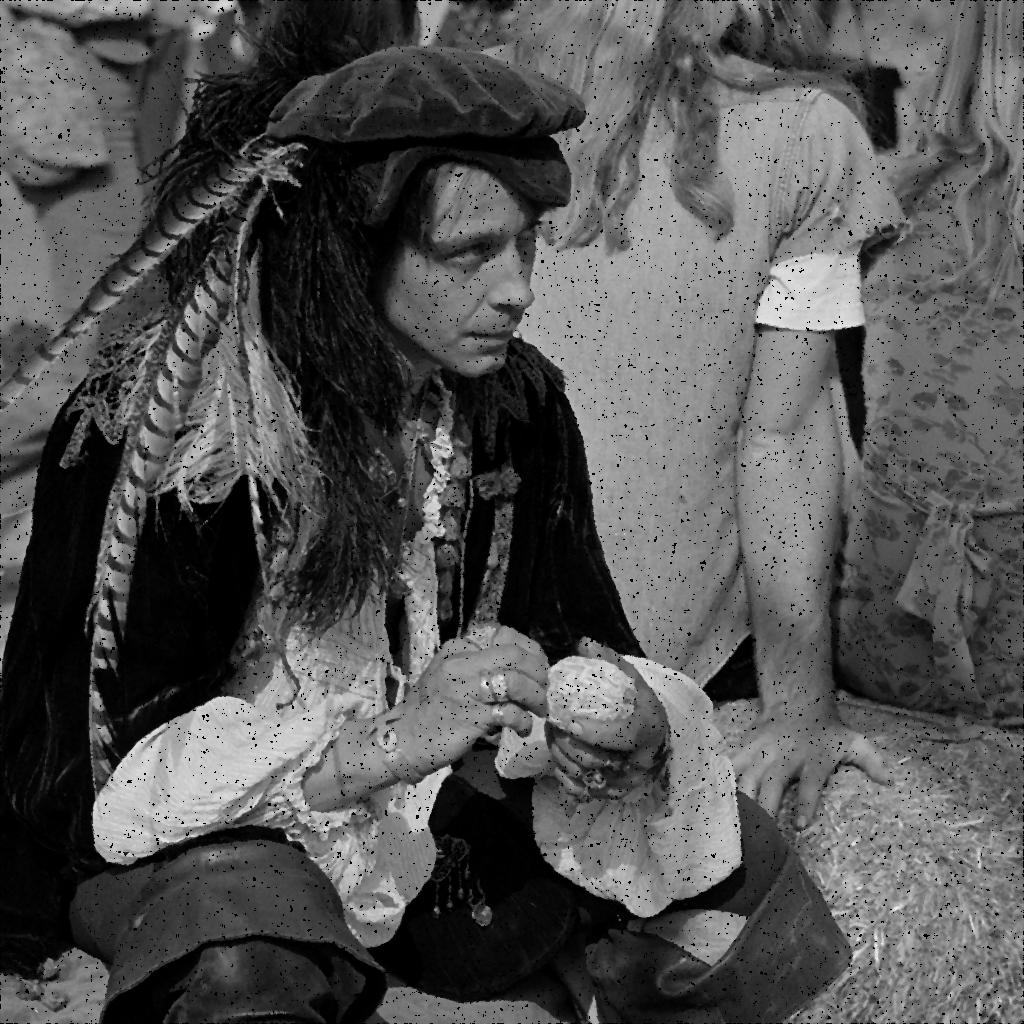
\includegraphics[width=10cm]{MeanFiltering.jpg}
\caption{Mean Filtering} \label{fig: Mean Filtering}
\end{figure}

\begin{figure}[h]
\centering
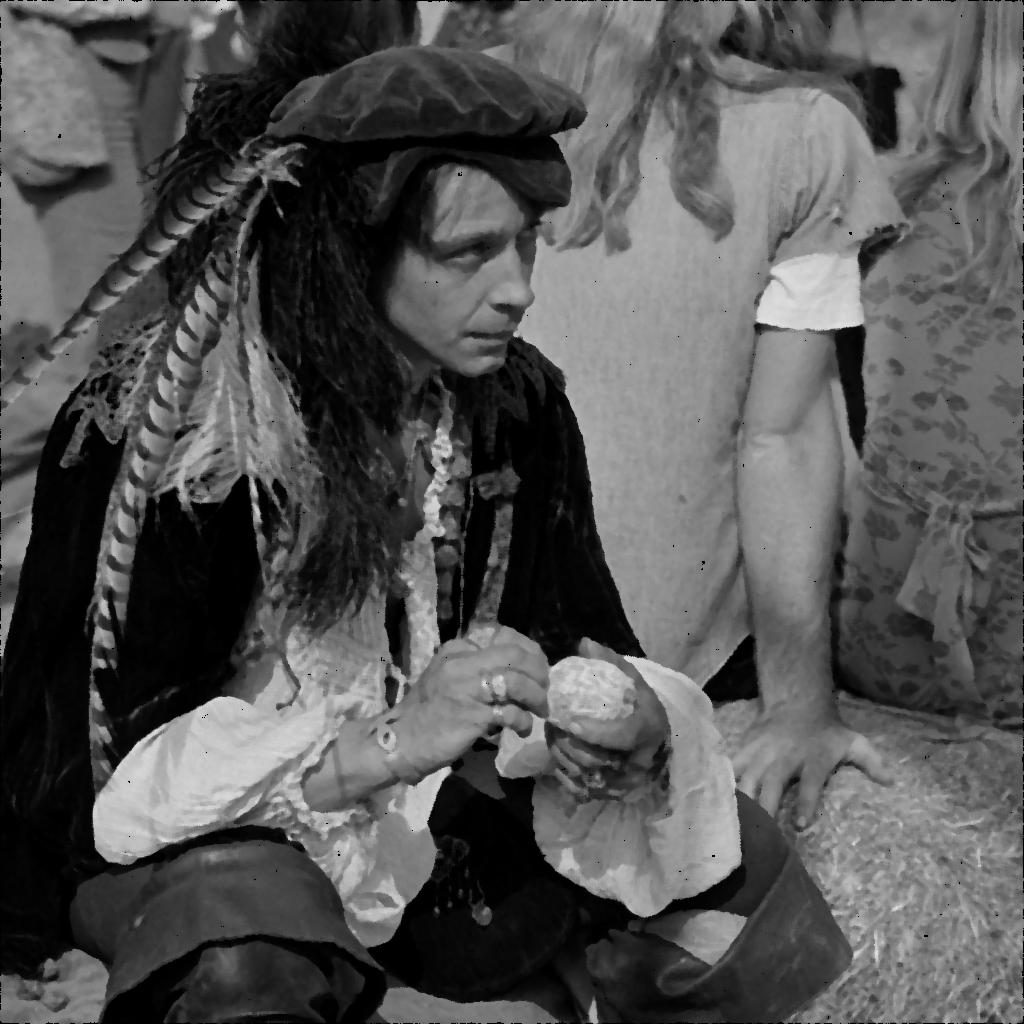
\includegraphics[width=10cm]{MedianFiltering.jpg}
\caption{Median Filtering} \label{fig: Median Filtering}
\end{figure}   

Median filter is a commonly used nonlinear filter. The basic process is to select the median of each pixel in a neighborhood of pixels to be processed instead of the pixel to be processed. The main principle is that the gray value of the pixel is close to the surrounding pixel, and the isolated noise point will not be the median, so the median filter can eliminate the salt and pepper noise very well.
In addition, compared with the mean filter, the median filter can effectively protect the boundary information of the image while eliminating the noise, and it will not cause a great blur to the image.
The formula is as follows:
\begin{equation}
  \hat{f}(x,y) = median_{(s,t)\in {S_{xy}}}\left\{g(s,t)\right\}
\end{equation}

We found in the test, the effect of median filter are greatly influenced by the filter window size, in eliminating noise and protect the image detail there exists a contradiction: the filter window is lesser, can very good protection in the image details, but for the noise of the filtering effect is not very good; On the contrary, the filter with larger window size has better noise filtering effect, but it can cause certain blurring to the image.
In addition, according to the principle of median filter, if the number of noise points in the filter window is greater than the number of pixels in the entire window, the median filter can not filter out the noise very well.

Therefore the median filter mentioned above, under the condition of noise density is not very big (according to the experience, the probability of the presence of the noise is less than 0.2), the effect is good.

\begin{figure}[h]
\centering
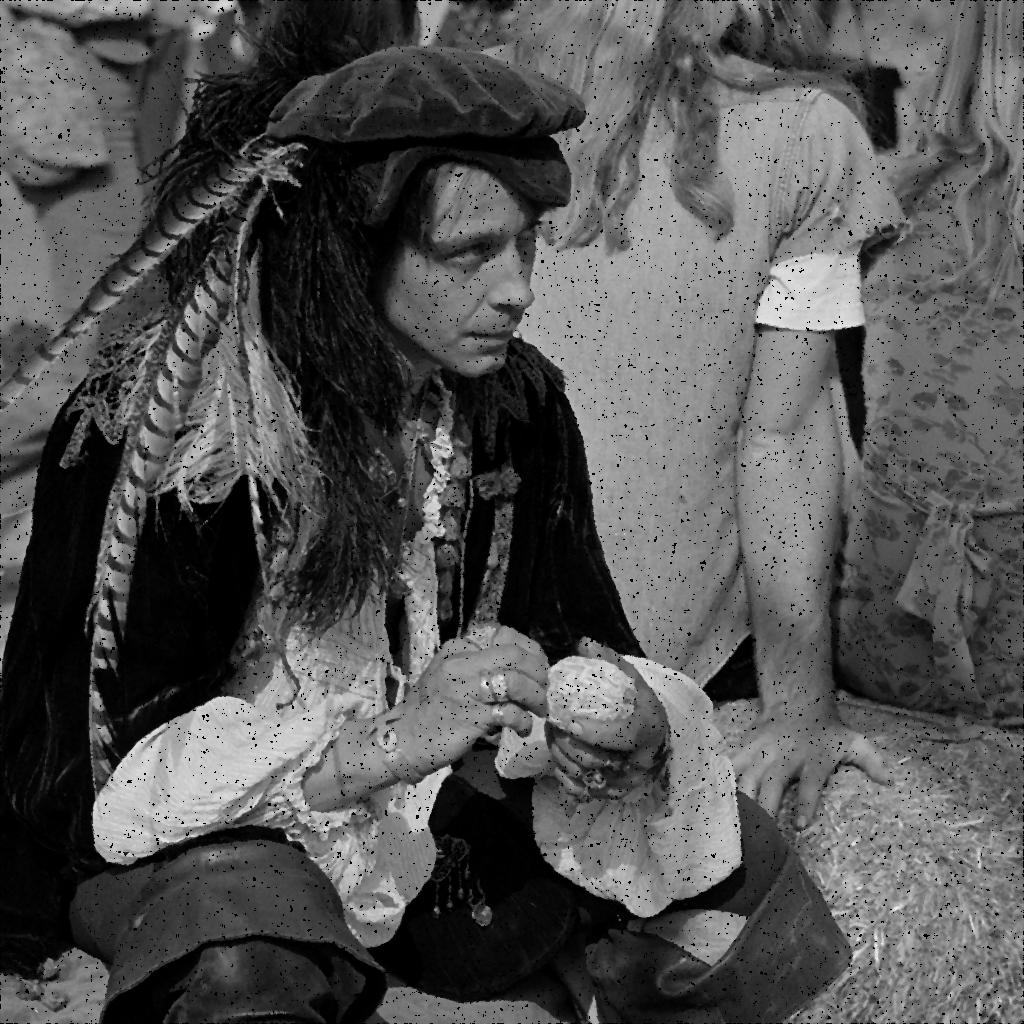
\includegraphics[width=7cm]{33m.jpg}
\caption{3X3Median Filtering} \label{fig: 3X3Median Filtering}
\end{figure} 

\begin{figure}[h]
\centering
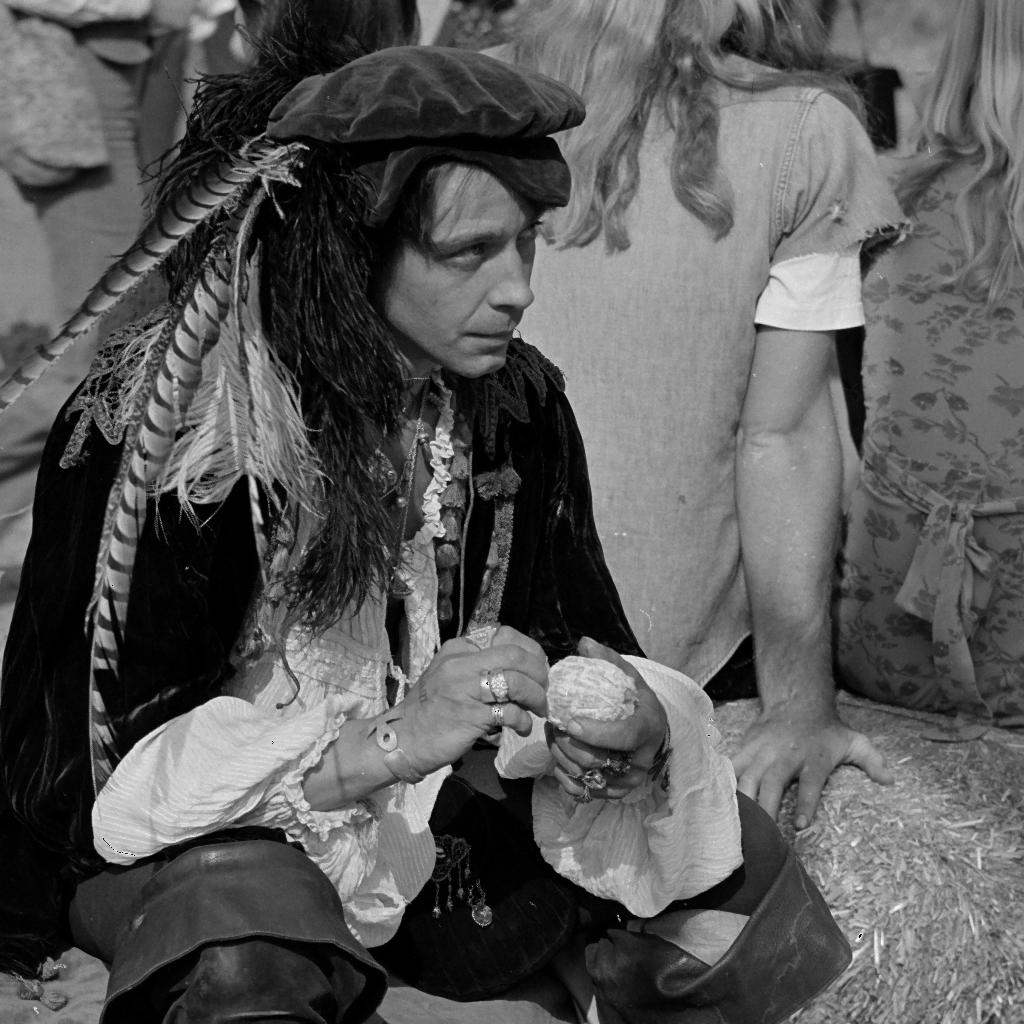
\includegraphics[width=7cm]{33a.jpg}
\caption{Adaptive Median Filtering} \label{fig: Adaptive Median Filtering}
\end{figure} 
  
So we finally chose the adaptive median filter. According to predefined condition, in the process of filtering, dynamic change the window size of the filter, as well as figure out whether the current pixel noise according to certain conditions. At the same time, it will judge whether the current pixel is noisy according to certain conditions, and if it is,replace the current pixel with the median value; If not, the pixel value is not changed.

Adaptive median filter has three purposes:
\begin{itemize}
  \item Filter the salt and pepper noise.
  \item Smooth other non-impulsive noise.
  \item Protect the details of the image as much as possible to avoid thinning or roughing the edges of the image.
\end{itemize}

\subsubsection{Model interpretation}
The adaptive filter can not only filter the salt and pepper noise with higher probability, but also can better protect the details of the image,which is not possible with conventional median filter.
The adaptive median filter also requires a rectangular window $S_{xy}$, which is different from the conventional median filter that the size of the window will change during the filtering process.
It is important to note that the output of the filter is a pixel value, which is used to replace the pixel values at the point (x,y), and the point (x,y) is the central location of the filter window.

The adaptive median filter has two processing processes: A and B:

\emph{A}:

$A_1 = Z_{med}−Z_{min}$;   
$A_2 = Z_{med}−Z_{max}$.  
If $A_1 > 0$ and $A_2 < 0$, jump to B;
Otherwise, increase the size of the window.
If the size of the rear window is less than or equal to $S_{max}$, repeat the A process.
Otherwise, output $Z_{med}$.

\emph{B}:

$B_1 = Z_{xy}−Z_{min}$;  
$B_2 = Z_{xy}−Z_{max}$.  
If $B_1>0$and $B_2<0$ , then the output is $Z_{xy}$.
Otherwise output $Z_{med}$.


The purpose of process A is to determine whether the median $Z_{med}$ is noise in the current window.If $Z_{min} < Z_{xy} < Z_{max}$, the median $Z_{med}$is not noise, then it turn to the process B testing to test whether the pixel Zxy of the center position of the current window is a noise point.
If $Z_{min} < Z_{xy} < Z_{max}$, $Z_{xy}$ is not a noise, then the filter output $Z_{xy}$; If the above conditions are not met, $Z_{xy}$ is determined to be noise, and the output value is $Z_{med}$ ($Z_{med}$ is not noise in A).

If $Z_{med}$ does not meet the condition $Z_{min}<Z_{med}<Z_{max}$, the median $Z_{med}$ is a noise. In this case, the window size of the filter needs to be enlarged, and the median value of a non-noise point is searched in a larger scope until it is found, then jump to B; Or, the size of the window reaches the maximum value, then returns the median found and exits.

The total flow chart is as follows:
[图  自适应中值滤波器总流程图]

From the above analysis, it can be seen that the probability of noise is low, and the adaptive median filter can get the results quickly, without the need to increase the size of the window. On the other hand, the probability of noise is higher, and it needs to increase the window size of the filter, which is the characteristic of a median filter which requires a larger filter window size when meets more noise points.

\section{Analysis of Results}
\subsection{Problem 1}

\subsection{Problem 2}

\section{Model Evaluation}
\subsection{Model \Rmnum{1}}
\subsubsection{Advantages}
\begin{itemize}
  \item According to the quantization factors, the compression ratio of different levels can be selected, which can be better adapted to many scenarios.
  \item It supports 24bit true color, and can be used for images and grayscale images of RGB channels.
  \item The model can be used for rectangular and square images, and the length of the picture does not affect the coding effect.
  \item The RLE part simplifies the encoding, and only the special encoding of 0 makes it perform better in high compression ratio.
  \item The compressed signal-to-noise ratio is good, and the image content is not seriously affected by the high compression ratio.
\end{itemize}

\subsubsection{Disadvantages}
\begin{itemize}
  \item The 0-RLE part simplifies the coding and requires more storage than the normal RLE in the case of low compression ratio.
  \item The quantification factor should not be less than 0.5, otherwise some pictures cannot be compressed.
\end{itemize}

\subsection{Model \Rmnum{2}}
\subsubsection{Advantages}
\begin{itemize}
  \item The model is simple and easy to implement.
  \item The model can adapt to the image of different loss under the same loss type.
\end{itemize}

\subsubsection{Disadvantages}
\begin{itemize}
  \item Unable to adapt well to other types of losses.
  \item For this problem, there are more external data introduced, and fewer things are created by oneself.
\end{itemize}

\subsubsection{Improvement}
\begin{itemize}
  \item we can consider adding image quality automatic recognition, which automatically identifies the type of image loss, and then select the best treatment method suitable for this type.
\end{itemize}

\begin{thebibliography}{99}
\bibitem{1} D.~E. KNUTH   The \TeX{}book  the American
Mathematical Society and Addison-Wesley
Publishing Company , 1984-1986.
\bibitem{2}Lamport, Leslie,  \LaTeX{}: `` A Document Preparation System '',
Addison-Wesley Publishing Company, 1986.
\bibitem{3}\url{http://www.latexstudio.net/}
\bibitem{4}\url{http://www.chinatex.org/}
\end{thebibliography}

\begin{appendices}

\section{First appendix}

\lipsum[13]

Here are simulation programmes we used in our model as follow.\\

\textbf{\textcolor[rgb]{0.98,0.00,0.00}{Input matlab source:}}
\lstinputlisting[language=Matlab]{./code/mcmthesis-matlab1.m}

\section{Second appendix}

some more text \textcolor[rgb]{0.98,0.00,0.00}{\textbf{Input C++ source:}}
\lstinputlisting[language=C++]{./code/mcmthesis-sudoku.cpp}

\end{appendices}
\end{document}

%% 
%% This work consists of these files mcmthesis.dtx,
%%                                   figures/ and
%%                                   code/,
%% and the derived files             mcmthesis.cls,
%%                                   mcmthesis-demo.tex,
%%                                   README,
%%                                   LICENSE,
%%                                   mcmthesis.pdf and
%%                                   mcmthesis-demo.pdf.
%%
%% End of file `mcmthesis-demo.tex'.
